\chapter{Раздел по охране труда}

\section{Гигиеничекие требования к персональным ЭВМ и организации работы}

Разработка ПО требует длительного взаимодействия с вычмслительными системами. Работа с ПЭВМ связана с рядом вредных и опасных факторов, таких как статическое электричество, рентгеновское излучение, электромагнитные поля, блики отраженный свет, ультрафиолетовое излучение. При длительном воздействии на организм эти факторы негативно влияют на здоровье человека.

\subsection{Микроклимат}

Работа как программиста, так и пользователя относится к категории 1а, поскольку не предполагает больших физических усилий. Нормы, установленные СанПиН 2.2.2/2.4.1340-03 для категории работ 1а приведены в таблице~\ref{tab:microclimate}.

\begin{table}[ht]
\caption{Нормы микроклимата}
\begin{tabular}{|l|c|c|c|c|c|c|}
\hline
\multirow{2}{*}{Период год} & \multicolumn{2}{l|}{Температура, $^\circ \mbox{C}$} & \multicolumn{2}{l|}{Влажность, \%} & \multicolumn{2}{l|}{Скорость воздуха, м/с} \\
\cline{2-7}
&Оптим.&Допуст.&Оптим.&Допуст.&Оптим.&Допуст.\\
\hline
Холодный &22--24&21--25&40--60&75&0.1&0.1\\
\hline
Теплый &23--25&22--28&40--60&55 при 28$^\circ \mbox{C}$&0.1&0.1\\
\hline 
\end{tabular}
\label{tab:microclimate}
\end{table}

Вредным фактором при работе с ЭВМ является также запыленность помещения. Этот фактор усугубляется влиянием на частицы пыли электростатических полей персональных компьютеров.

Для устранения несоответствия параметров указанным нормам проектом предусмотренно использование системы кондиционирования как наиболее эффективного и автоматически функционирующего средства.

Нормы установленные содержания в воздухе положительных и отрицательной ионов, установленные СанПиН 2.2.4.1294--03, приведены в таблице~\ref{tab:ions}.

\begin{table}[ht]
\caption{Уровни ионизации воздуха при работе на ПЭВМ}
\begin{tabular}{|l|c|c|}
\hline
\multirow{2}{*}{Уровни} & \multicolumn{2}{l|}{Число ионов в кубометре воздуха}\\
\cline{2-3}
&$n^+$&$n^-$\\
\hline
Минимально необходимое & 400 & 600 \\
\hline
Оптимальное & 1500--3000 & 3000--5000 \\
\hline
Максимально допустимое & 50000 & 50000 \\
\hline
\end{tabular}
\label{tab:ions}
\end{table}

Для обеспечения требуемых уровней предусмотренно использование системы ионизации Сапфир-4А.

\subsection{Шум и вибрации}

Уровень шума на рабочем месте программиста не должен превышать 50 дБА, а уровень вирации не должен превышать норм становленных СанПиН 2.2.2.542--96 (см. таблицу~\ref{tab:vibro}).

\begin{table}[ht]
\caption{Допустимые нормы вибрации на раочих местах с ПЭВМ}
\begin{tabular}{|c|c|c|}
\hline
\parbox{0.4\textwidth}{ Среднегеометрические частоты\\октавных полос, Гц}& \multicolumn{2}{l|}{Допустимые значения по виброскорости}\\
\cline{2-3}
&м/c &дБ\\
\hline
2  & $4.5\times10$ & 79 \\
\hline
4  & $2.2\times10$ & 73 \\
\hline
8  & $1.1\times10$ & 67 \\
\hline
16  & $1.1\times10$ & 67 \\
\hline
31.5 & $1.1\times10$ & 67 \\
\hline
63  & $1.1\times10$ & 67 \\
\hline
\parbox{0.4\textwidth}{ Корректированные значения\\и их уровни в дБ}& $2.0\times10$ & 72\\
\hline
\end{tabular}
\label{tab:vibro}
\end{table}

При разработке ПО внутренними источниками шума являются вентиляторы, а также принтеры и другие перефферийные устройства ЭВМ. Внешние источники шума~--- прежде всего, шум с улицы и из соседних помещений. Постоянные внешние источники шума, превышающего нормы, отсутствуют.

Для устранения превышения нормы проектом предусмотрено применение звукопоглощающих материалов для облицовки стен и потолка помещения, в котором осуществляется работа с вычислительной техникой.

\subsection{Освещение}

Наиболее важным условием эффективной раоты программитов и пользователей является соблюдение оптимальных параметров системы освещения в рабочих помещениях.

Естественное освещение осуществляется через светопроемы, ориентированные в основном на север и северо-восток (для исключения попадания прямых солнечных лучей на экраны компьютеров) и обеспечивает коэффициент естественной освещенности (КЕО) не ниже 1.5\%.

В качестве искуственного освещения проектом предусмотрено использование системы общего освещения. в соответствии с СанПин 2.2.2/2.4.1340--03 освещенность на поверхнности рабочего стола должна находиться в пределах 300--500 лк. Разрешается использование светильников местного освещения для работы в документами (при этом светильники не должны создавать блики на поверхности экрана).

Правильное расположение рабочих мест относительно источников освещения, отсутствие зеркальных поверхностей и использование матовых материалов ограничивает прямую (от источников освещения) и отраженную (от рабочих поверхностей) блескость. При  этом яркость светящихся пооверхностей не привышает $200 \frac{\text{кд}}{\text{м}^2}$, яркость бликов на экране ПЭВМ не превышает $40 \frac{\text{кд}}{\text{м}^2}$, и яркость потолка не превышает $200 \frac{\text{кд}}{\text{м}^2}$.

В соответствии с СанПинН 2.2.2/2.4.1340--03 проектом предусмотрено использование люминисцентных ламп типа ЛБ в качестве источников света при искуственном освещении. В светильниках допускается применение ламп накаливания. Применение газоразрядных ламп в светильниках общего и местного освещения обеспечивает коэффициент пульсации не более 5\%.

Таким образом, проектом обеспечиваются оптимальные условия освещения рабочего помещения.

\subsection{Рентгеновское излучение}

В соответствии с СанПиН 2.2.2/2.4.1340-03 проектом предусмотрено использование ПЭВМ, конструкция которого обеспечивает мощность экспозиционной дозы рентгеновского излучения в любой точке на расстоянии 0.5 м. от экрана и корпуса не более 0.1 мбэр/час (100 мкР/час). Результаты сравнения норм излучения приведены в таблице~\ref{tab:rentgen}.

\begin{table}[ht]
\caption{Сравнение норм рентгеновского излучения в различных стандартах}
\begin{tabular}{|l|c|}
\hline
& Допустимое значение мкР/час, не более \\
\hline
СанПиН 2.2.2/2.4.1340-03 & 100 \\
\hline
ТСО-99 & 500 \\
\hline
MPR II & 500\\
\hline
\end{tabular}
\label{tab:rentgen}
\end{table}

Как видно из таблицы, стандарты MPR II и ТСО--99 предъявляют менее жесткие требования к рентгеновскому излучению, чем СанПиН. Но при соблюдении оптимального расстояния между пользователем и монитором дозы рентгеновского излучения не опасны для большнства людей.

\subsection{Неионизирующие электромагнитные излучения}

Допустимые значения параметров неионизирующих излучений в соответствии с СанПин 2.2.2/2.4.1340-03 приведены в таблицах~\ref{tab:U} и~\ref{tab:ro}.

\begin{table}[ht]
\caption{Предельно допустимые значения напряженности электрического поля}
\begin{tabular}{|c|c|}
\hline
Диапазон частот& Допустимые значения \\
\hline
5 Гц -- 2 кГц & 25 В/м \\
\hline
2 -- 400 кГц& 2.5 В/м \\
\hline
\end{tabular}
\label{tab:U}
\end{table}

\begin{table}[ht]
\caption{Предельно допустимые значения плотности магнитного потока}
\begin{tabular}{|c|c|}
\hline
Диапазон частот& Допустимые значения \\
\hline
5 Гц -- 2 кГц & 250 нТл \\
\hline
2 -- 400 кГц& 5 нТл \\
\hline
\end{tabular}
\label{tab:ro}
\end{table}

Величина поверхностного электрического потенциала не должна превышать 500 В.

Мониторы, используемые в настоящее время, удовлетворяют более жестким нормам MPR II, а значит и СанПиН.

\subsection{Визуальные параметры}

Неправильный выбор визуальных эргономических параметров приводит к ухудшению здоровья пользователей, быстрой утомляемости, раздражительности. В связи с этим, проектом предусмотрено, что конструкция вычислительной системы и ее эргономические параметры обеспечивают комфортное и надежное считывание иныформации. Требования к визуальным параметрам, их внешнему виду, дизайну, возможности настроцки представлены в СанПиН 2.2.2/2.4.1340--03. Визуальные эргономические параметры монитора и пределы из изменений приведены в таблице~\ref{tab:ergonom}.

\begin{table}[ht]
\caption{Визуальные эргономические параметры ВДТ и пределы из изменений}
\begin{tabular}{|p{0.5\textwidth}|c|c|}
\hline
\multirow{2}{*}{Наименование параметров} & \multicolumn{2}{c|}{Пределы значений параметров}\\
\cline{2-3}
&не менее&не более\\
\hline
Яркость экрана (фона), $\frac{\text{кд}}{\text{м}^2}$ (измеренная в темноте) &35&120\\
\hline
Внешняя освещенность экрана, лк &100&250\\
\hline
Угловой размер экрана, угл.мин. &16&60\\
\hline
\end{tabular}
\label{tab:ergonom}
\end{table}

Для выполнения этих требований проектом предусмотренно использование современных мониторов, имеющих достаточно широкий набор регулируемых параметтров.  В частности, для удобного считывания информации реализована возможность настройки положения монитора по горизонтали и вертикали. Мониторы оснащены специальными устройствами и средствами настройки ширины, высоты, яркости, контраста и разрешения изображения. кроме того, в современных мониторах зерно изображения имеет размер в пределах 0.27 мм, что обеспечивает высокую четкость и непрерывность изображения. Наконец, на поверхность дисплея нанесено матовое покрытие, чтобы избавиться от солнечных бликов.

\section{Расчет искусственного освещения}

При расчете освещенности от светильников общего равномерного освещения наиболее часто применяют метод расчета по светтовому потоку. При расчете освещения по этому методу необходимое количество светильников для освещения оабочего места расчитывается по формуле:

\begin{equation}
\label{f:lightsCount}
N = \frac{E_{min}\cdot S\cdot K}{F_\text{Л} \cdot \text{З} \cdot z \cdot h}
\end{equation}

где $E_{min}$~--- нормируемая минимальная освещенность; $S$~--- площадь помещения, $\text{м}^2$; $F_\text{Л}$~--- ветовой поток лампы, лк; $K$~--- коэффициент запаса; $z$~--- коэффициент неравномерности освещения (для люминисцентных ламп~---1.1); $h$~--- коэффициент использования светового потока в долях единицы.

$E_{min}$ определяется на основании нормативного документа СНиП23--05--95. В соответствии с произведенным выбором в предыдущем разделе, для работы программиста $E_{min}=300$ лк (общее освещение).

Работы, производятся в помещении, требуют различения цветных объектов при невысоких требованиях к цветоразличению, поэтому в качестве источника освещения была выбрана лампа люминисцентная холодно-белая (ЛХБ), 1940 лк, 30 Вт. В помещениях общественных и жилых зданий с нормальными условиями среды: К=1.4.

Для люминисцентных ламп коэффициент неравномерности освещения Z=1.1.

Коэффициент использования h зависит от типа свтильника, от коэффициентов отражения потолка $\rho_\text{П}$, стен $\rho_\text{С}$, расчетной поверхности $\rho_\text{Р}$ и индекса помещения.

Высота подвеса над рабочей поверностю Нр=3 м. Размеры помещения А=3.5 м, В=3 м. Определим индекс по мещения по формуле:

\begin{equation}
\phi = \frac{A \cdot B}{H_P \cdot (A + B)} = \frac{3.5 \cdot 3}{s \cdot (3.5 + 3)} = 0.54
\end{equation}

Для светлого фона примем:$\rho_\text{П} = 70$ $\rho_\text{С} = 50$ $\rho_\text{Р} = 10$. h = 59\%.

Освещение проектируется при помощи светильников ОДОР с минимальной освещенностью $E_{min}=300$ лк, P=40 Вт. Число ламп в ОДОР равно 2. Необходимое число светильников для данной комнаты:

\begin{equation}
N = \frac{300 \cdot 9 \cdot 1.4}{1940 \cdot 0.59 \cdot 1.1 \cdot 2} = 2 \text{шт}
\end{equation}

Общее количество ламп $n = 2\times2=4$ шт. Длина светильника ОДОР=1.26 м. Поскольку длина помещения 3 м, то светильники помещаются в два ряда. схема размещения светильников показана на Рисунке~\ref{fig:light}.

\begin{figure}
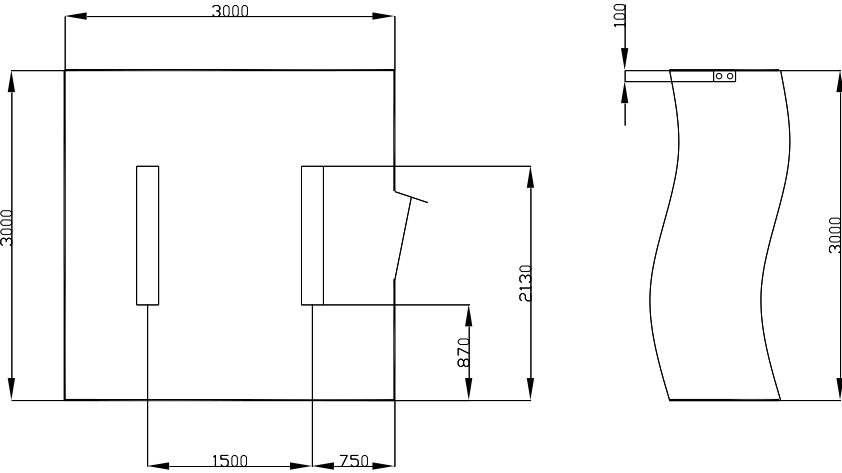
\includegraphics[width=\textwidth]{inc/light.png}
\caption{План размещения светильников в машинном зале}
\label{fig:light}
\end{figure}

Суммарная мощность светильников: $30\cdot4=160$ Вт. Сумарный световой поток: $1940\cdot4=7760$ лм.

Режим труда и отдыха должен зависеть от характера работы: при вводе данных, раедактировании программ, чтении информации с экрана непрерывная продолжительность работы с монитором не должна превышать 4 часов. При 8 часовом рабочем дне, через кадый час рпботы необходимо проводить перерыв 5--10 минут, а каждые два часа перерыв в 15 мин.
